\section{Theorie}
\usetikzlibrary{circuits.ee.IEC}
\label{sec:Theorie}

Das Ziel einer Brückenschaltung ist es oft, Widerstände oder 
physikalische Größen, die sich als Widerstände darstellen lassen, zu messen 
(dazu gehören auch komplexe Widerstände).
Mit Hilfe der Krichhoffschen Regeln lassen sich diese Widerstände durch die 
Speisespannung $U_s$ und die Brückenspannung $U$ darstellen.

Das erste Krichhoffsche Gesetz ist dabei die sogenannte Knotenregel. 
Sie besagt, dass die Summe der zufließenden Ströme der Summe der
abfließenden Ströme entspricht. 
\begin{equation}
\sum_{k} I_k = 0
\end{equation}
Anschaulich wird diese Regel an dem Beispiel in Abbildung 1, in der gilt, dass
\begin{equation}
I_1=I_2+I_3
\end{equation}

\begin{figure}
    \centering
    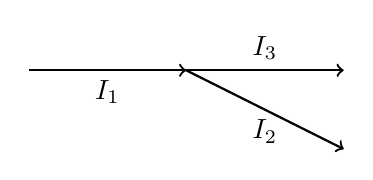
\begin{tikzpicture}
    \draw [thick, ->] (10, 0) -- +(2, 0) node[midway,   below] {$I_1$};
    \draw [thick, ->] (12, 0) -- +(2, -1) node[midway, below] {$I_2$}; 
    \draw [thick, ->] (12, 0) -- +(2, 0) node[midway, above] {$I_3$};
    \end{tikzpicture}
    \caption{Knotenregel}
    \label{fig:Knotenregel}
\end{figure}

Die zweite Krichhoffsche Regel wird als Maschenregel bezeichnet. Sie besagt, dass 
in einer geschlossenen Masche einer elektrischen Schaltung die Summe aller 
Spannungen null ergeben muss.
\begin{equation}
\sum_{i=1}^n  U_i = 0
\end{equation}

\begin{figure}
    \centering
    \begin{tikzpicture}[circuit ee IEC, font=\sffamily]
    \draw (0,0) to [resistor={info={$R_1$}}] (4, 0);
    \node[current direction={red, info={[red]\texttt{\itshape{I}}}}] at (0.5,0) {};
    \draw (4, 0) -- (4, -2);
    \draw (0, -2) to [resistor={info={$R_2$}}] (4, -2);
    \draw (0,0) to [battery={info'={$U_s$}}] (0,-2);
    \end{tikzpicture}
    \caption{Maschenregel}
    \label{fig:Maschenregel}
\end{figure}

Hier gilt demnach:
\begin{equation}
U_s=I\cdot R_1+I\cdot R_2
\end{equation}

Um eine unbekannte Größe zu ermitteln, wird eine Brückenschaltung benötigt,
deren prinzipieller Aufbau in Abbildung 3 zu sehen ist. 

\begin{figure}
    \centering
    \begin{tikzpicture}[circuit ee IEC, font=\sffamily, scale=0.75]
    \draw (0,0) to [battery={info'={$U_s$}}] (0,-10);
    \draw (0, 0) -- (6, 0);
    \draw (6, 0) -- (6, -1);
    \node[contact] at (6,-1) {};
    \draw (3, -1) -- (9, -1);
    \draw (3, -1) to [resistor={info={$R_1$}}] (3, -5);
    \draw [->] (3, -1) -- +(0, -1) node[midway, left] {$I_1$};
    \draw (9, -1) to [resistor={info={$R_3$}}] (9, -5);
    \draw [->] (9, -1) -- +(0, -1) node[midway, right] {$I_3$};
    \coordinate[label=left:$C$] (C) at (3, -5);
    \node[contact] at (3,-5) {};
    \coordinate[label=right:$D$] (D) at (9, -5);
    \node[contact] at (9,-5) {};
    \draw (3, -5) -- (5.5, -5);
    \draw (6.5, -5) -- (9,-5);
    \coordinate[label=above:$A$] (A) at (5.5, -5);
    \node[contact] at (5.5,-5) {};
    \coordinate[label=above:$U$] (U) at (6, -5.25);
    \coordinate[label=above:$B$] (B) at (6.5, -5);
    \node[contact] at (6.5,-5) {};
    \draw (3, -5) to [resistor={info={$R_2$}}] (3, -9);
    \draw [->] (3, -7.5) -- +(0, -1) node[midway, left] {$I_2$};
    \draw (9, -5) to [resistor={info={$R_4$}}] (9, -9);
    \draw [->] (9, -7.5) -- +(0, -1) node[midway, right] {$I_4$};
    \draw (3, -9) -- (9, -9);
    \node [contact] at (6,-9) {};
    \draw (6, -9) -- (6, -10);
    \draw (0, -10) -- (6, -10);
    \end{tikzpicture}
    \caption{Prinzipielle Brückenschaltung}
    \label{fig:Prinzipielle Brückenschaltung}
\end{figure}

Bei einigen Brückenschaltungen ist es zweckmäßig komplexe Widerstandsoperatoren
zu benutzen. Ein komplexer Widerstand lässt sich im Allgemeinem darstellen durch

\begin{equation}
Z=R+iX
\end{equation}

Dabei bezeichnet $X$ den Blindwiderstand und $R$ den Wirkwiderstand.
Nach der Knotenregel (1) gilt in der Abbildung 3: 
\begin{gather}
I_1 = I_2 \\
I_3 = I_4 
\end{gather}

Die Anwendung der Maschenregel führt zu den beiden Ausdrücken:
\begin{gather}
U = -Z_1\cdot I_1 + Z_3\cdot I_3 \\
-U = -Z_2\cdot I_2 + Z_4\cdot I_4
\end{gather}

Einsetzen von (6) und (7) in (9) führt zu:

\begin{equation}
-U = -Z_2\cdot I_1 + Z_4\cdot I_3
\end{equation}

Umformen von (8) und (10) zu $I_3$, gleichsetzen und umformen zu $U$ führt zu:

\begin{equation}
U = \frac{Z_2\cdot Z_3 - Z_1\cdot Z_4}{Z_3 + Z_4} \cdot I_1
\end{equation}

Nach der Maschenregel (3) gilt außerdem:

\begin{equation}
U_s = I_1\cdot (Z_1 + Z_2)
\end{equation}

Durch diese kombinierte Anwendung der Knoten- (1), Maschenregel (3)
und Umformung von (12) zu $I_1$ und einsetzen in (11) gelangt man 
schließlich zu dem Ausdruck: 

\begin{equation}
U = \frac{Z_2\cdot Z_3 - Z_1\cdot Z_4}{(Z_3 + Z_4)\cdot (Z_1 + Z_2)} \cdot U_s
\end{equation}

Die Brückenspannung verschwindet dann, wenn der Ausdruck über dem 
Bruch null wird. Dies ist der Fall, wenn
\begin{equation}
Z_1\cdot Z_4 = Z_2\cdot Z_3
\end{equation}

Dies bezeichnet man als abgeglichene Brücke. Ist also einer der 
Widerstände unbekannt, kann man einen der anderen solange variieren,
bis die Brückenspannung komplett verschwindet und dann beispielsweise 
$Z_1$ berechnen:

\begin{equation}
Z_1 = \frac{Z_2\cdot Z_3}{Z_4}
\end{equation}

Handelt es sich allerdings um komplexe Widerstände müssen
die beiden Gleichungen:

\begin{gather}
R_1\cdot R_4 - X_1\cdot X_4 = R_2\cdot R_3 - X_2\cdot X_3 \\
R_1\cdot X_4 + R_4\cdot X_1 = R_2\cdot X_3 - R_3\cdot X_2 
\end{gather}

gleichzeitig erfüllt sein. Dementsprechend müssen zwei Widerstände
variiert werden bis die Brückenspannung null wird.

Die Impedanzen eines ohmschen Widerstands $R$, einer Induktivität $L$
und einer Kapazität $C$ sind gegeben durch: 

\begin{gather}
Z_R = R \\
Z_L = i\omega L \\
Z_C = \frac{-i}{\omega C}
\end{gather}

\cite{sample}
